%%%%%%%%%%%%%%%%%%%%%%%%%
\section{\label{sec:rhs_gibbs}Unbiased Gibbs ensemble trials}
%%%%%%%%%%%%%%%%%%%%%%%%%

In the Gibbs ensemble, separate domains are simulated for which chemical and mechanical equilibrium at constant temperature is established between them \cite{panagiotopoulos_direct_1987}, although chemical equilibrium is sufficient to enforce mechanical equilibrium \cite{panagiotopoulos_adsorption_1987}.
For notational convenience, we will consider only two domains such that the total volume, $V=V_1+V_2$, is the sum of two volumes and the total number of particles of type $i$, $N_i$, is $N_{i1} + N_{i2}$.
Volume changes require scaling, as described in Section \ref{sec:rhs_npt}, and the particle positions must be expressed in terms of the scaled coordinates.
We do not consider constant-pressure Gibbs ensemble in this work \cite{panagiotopoulos_phase_1988}.
Although recent studies show that Gibbs (and all other) ensemble simulations may utilize a shell particle \cite{hatch_theory_2024}, we consider only the application of a shell particle in the $NPT$ ensemble in this article.

The probability of a microstate in the Gibbs ensemble is then given by \cite{panagiotopoulos_direct_1987, frenkel_understanding_2002, hatch_theory_2024},
\begin{equation}
\Pi \propto \frac{1}{\Lambda_i^{ND}}V_1^{N_{i1}}V_2^{N_{i2}} e^{-\beta (U_1+U_2)} \diff\mathbf{s}^{N} \diff V_1 \diff V_2.
\label{eq:rhs_gibbs_pi}
\end{equation}
For particle transfer between domains while holding the volume of each domain fixed, the ratio of microstates in the Gibbs ensemble with particle transfer, the first ratio of Eq.~\ref{eq:detailed_balance}, is given by
\begin{equation}
\frac{\Pi_{n}}{\Pi_{o}} = V_1^{N_{ni1}-N_{oi1}} V_2^{N_{ni2}-N_{oi2}}e^{-\beta\Delta (U_1+U_2)},
\label{eq:rhs_gibbs_particle}
\end{equation}
where $N_{ni1}$ and $N_{ni2}$ are the number of particles of type $i$ in the first and second domain, respectively, in the new microstate, while $N_{oi1}$ and $N_{oi2}$ are in the old microstate.

For volume transfer between domains while holding the number of particles in each domain fixed, the ratio of microstates in the Gibbs ensemble with volume transfer, the first ratio of Eq.~\ref{eq:detailed_balance}, is given by
\begin{equation}
\frac{\Pi_{n}}{\Pi_{o}} = \left(\frac{V_{n1}}{V_{o1}}\right)^{N_{i1}}\left(\frac{V_{n2}}{V_{o2}}\right)^{N_{i2}}e^{-\beta\Delta (U_1+U_2)},
\label{eq:rhs_gibbs_volume}
\end{equation}
where $V_{n1}$ and $V_{n2}$ are the volume of the first and second domain, respectively, in the new microstate, while $V_{o1}$ and $V_{o2}$ are in the old microstate.

%%%%%%%%%%%%%%%%%%%%%%%%%
\subsection{\label{sec:lhs_gibbs_particle}Gibbs ensemble with particle transfer trials}
%%%%%%%%%%%%%%%%%%%%%%%%%

In this example, consider particle transfers between two domains, as illustrated in Fig.~\ref{fig:gibbs_particle}.
Particle transfers are conducted similarly to a simultaneous insertion in one domain and deletion in another domain, as described in Section~\ref{sec:lhs_insdel}.
The total number of particles remains constant, as well as the volumes of both systems and the temperature.

\begin{figure}
\begin{centering}
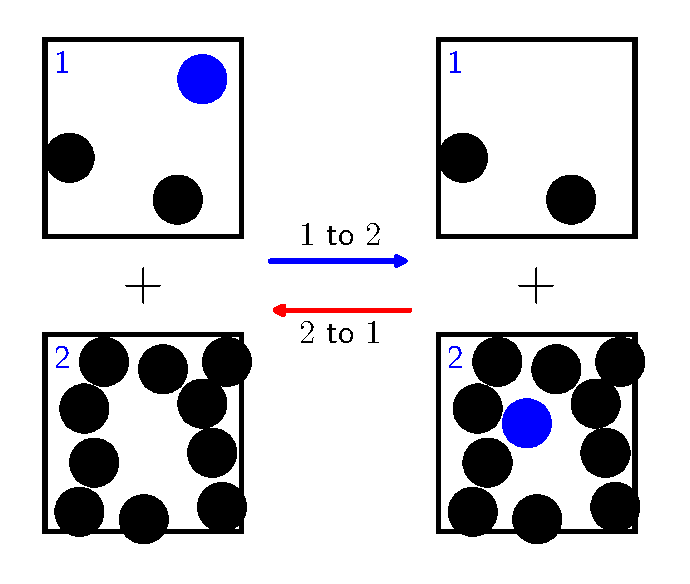
\includegraphics[width=6.5cm]{../figures/gibbs_particle.pdf}
\caption{
Gibbs ensemble transfer of the particle shown in blue from periodic domain $1$ to periodic domain $2$, and the reverse trial.
The total number of particles remains constant.
}
\label{fig:gibbs_particle}
\end{centering}
\end{figure}

Particle transfers between domains $1$ and $2$ in Gibbs ensemble MC proceed as follows.
With equal probability, domain $1$ is randomly chosen among all the domains to transfer a particle of a given type $i$.
A particle of type $i$ is then chosen for removal from domain $1$ with probability $1/N_{i1}$.
A particle of the same type is then added to domain $2$ at a random position selected uniformly within the volume, $V_2$.
The transition probabilities are summarized in Table~\ref{tab:lhs_gibbs_particle}, where $N_{i1}$ and $N_{i2}$ are the numbers of each type of particle in domains $1$ and $2$, respectively, before the trial is implemented.

\begin{table}
\begin{center}
\begin{tabular}{|c|c|}
 \hline
 \thead{Forward} & \thead{$\alpha_{o\rightarrow n}$} \\ [0.5ex]
 \hline
 Choose domain $1$ & $1/2$ \\
 \hline
 Choose particle of type $i$ in domain $1$ & $1/N_{i1}$ \\
 \hline
 Choose $\mathbf{s}_n$ in domain 2 & $\diff\mathbf{s}$ \\
 \hline
 Choose orientation of particle $i$ in domain 2 & $P_{\omega 2}\diff\boldsymbol{\omega}$ \\
 \hline\hline
 \thead{Reverse} & \thead{$\alpha_{n\rightarrow o}$} \\ [0.5ex]
 \hline
 Choose domain $2$ & $1/2$ \\
 \hline
 Choose particle of type $i$ in domain $2$ & $1/(N_{i2}+1)$ \\
 \hline
 Choose $\mathbf{s}_o$ in domain 1 & $\diff\mathbf{s}$ \\
 \hline
 Choose orientation of particle $i$ in domain 1 & $P_{\omega 1}\diff\boldsymbol{\omega}$ \\
 \hline
\end{tabular}
\caption{Gibbs ensemble particle transfer transition probabilities.}
\label{tab:lhs_gibbs_particle}
\end{center}
\end{table}

Using Table~\ref{sec:lhs_gibbs_particle} and substituting Eq.~\ref{eq:rhs_gibbs_particle} into Eq.~\ref{eq:detailed_balance}, the acceptance probability for the transfer of a particle of type $i$ from domain $1$ to domain $2$ as the forward transition is
\begin{equation}
\chi = \frac{N_{i1}}{N_{i2}+1}\left(\frac{V_2}{V_1}\right)\frac{P_{\omega 1}}{P_{\omega 2}}e^{-\beta(\Delta U_1 + \Delta U_2)}.
\label{eq:gibbs_transfer}
\end{equation}
If particles of type $i$ are rigid molecules and random orientations are chosen (or if isotropic), $P_{\omega 1}=P_{\omega 2}$.
Otherwise, $\frac{P_{\omega j}}{P_{\omega i}}$ is related to the Rosenbluth factors for configuration bias partial regrowth.
The transfer from domain $2$ to domain $1$ is identically derived by simply perturbing the indices $1$ and $2$.
Eq.~\ref{eq:gibbs_transfer} is tested in an ideal gas simulation demonstrated in Code Block~\ref{sim:gibbs_particle}, where the densities of the two domains should be equivalent \cite{hatch_theory_2024}.

\begin{figure}
\lstinputlisting[
language=Python,
label={sim:gibbs_particle},
caption={MC simulation of an ideal gas in the Gibbs ensemble with chemical equilibrium using Python 3 should yield two domains with equivalent density, and the statistics module is provided in Section~\ref{sec:block_av}.}
]{../codes/ideal_gas_gibbs_particle.py}
\end{figure}

%%%%%%%%%%%%%%%%%%%%%%%%%
\subsection{\label{sec:lhs_gibbs_volume}Gibbs ensemble with volume transfer trials}
%%%%%%%%%%%%%%%%%%%%%%%%%

In this example, consider volume transfers between two domains, as illustrated in Fig.~\ref{fig:gibbs_volume}.
Volume transfers are conducted similarly to a simultaneous expansion in one domain and correlated contraction in another domain, as described in Section~\ref{sec:lhs_dv}.
The total volume, $V=V_1+V_2$, remains constant, as well as the numbers of particles of each type in both systems and the temperature.

\begin{figure}
\begin{centering}
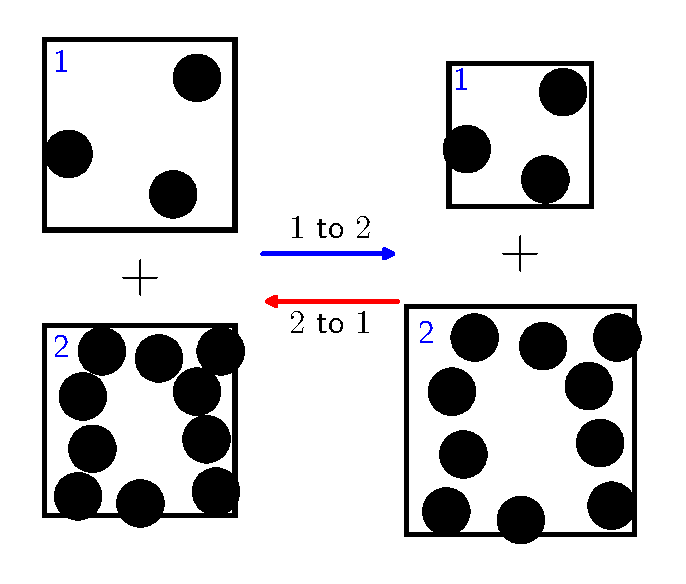
\includegraphics[width=6.5cm]{../figures/gibbs_volume.pdf}
\caption{
Gibbs ensemble transfer of volume from periodic domain $1$ to periodic domain $2$, and the reverse trial.
The total volume remains constant and the particle positions are scaled as described in Section~\ref{sec:lhs_dv}.
}
\label{fig:gibbs_volume}
\end{centering}
\end{figure}

Volume transfers between domains $1$ and $2$ in Gibbs ensemble MC proceed as follows.
As described in Section~\ref{sec:lhs_dv}, the positions of the particles and periodic boundary lengths are scaled by a factor of $(1+\Delta V/V_o)^{1/D}$ in each of $D$ dimensions, where $\Delta V$ is chosen as a random amount selected uniformly within $\pm\Delta V_{\mathrm{max}}$.
The scaling occurs with $-\Delta V$ for domain $1$, and $+\Delta V$ for domain 2, where $V_1$ and $V_2$ are the volumes of domains $1$ and $2$ before the scaling occurs.

\begin{table}
\begin{center}
% \begin{tabular}{|c|c|c|c|c|}
%  \cline{1-2}\cline{4-5}
%  \thead{Forward} & \thead{$\alpha_{o\rightarrow n}$} & & \thead{Reverse} & \thead{$\alpha_{n\rightarrow o}$}\\
%  \cline{1-2}\cline{4-5}
%  \makecell{Choose $\Delta V$} & \makecell{$\diff\mathbf{r}/(2\Delta V_{\mathrm{max}})$} & & \makecell{Choose $-\Delta V$} & \makecell{$\diff\mathbf{r}/(2\Delta V_{\mathrm{max}})$} \\
%  \cline{1-2}\cline{4-5}
\begin{tabular}{|c|c|}
 \hline
 \thead{Forward} & \thead{$\alpha_{o\rightarrow n}$} \\
 \hline
 \makecell{Choose $\Delta V$} & \makecell{$\diff\mathbf{r}/(2\Delta V_{\mathrm{max}})$} \\
 \hline\hline
 \thead{Reverse} & \thead{$\alpha_{n\rightarrow o}$}\\ [0.5ex]
 \hline
 \makecell{Choose $-\Delta V$} & \makecell{$\diff\mathbf{r}/(2\Delta V_{\mathrm{max}})$} \\
 \hline
\end{tabular}
\caption{Gibbs ensemble volume transfer transition probabilities.}
\label{tab:lhs_gibbs_volume}
\end{center}
\end{table}

Using the transition probabilities in Table~\ref{tab:lhs_gibbs_volume}, and substituting Eq.~\ref{eq:rhs_gibbs_volume} into Eq.~\ref{eq:detailed_balance}, the acceptance probability for the transfer of volume from domain $1$ to domain $2$ as the forward transition is
\begin{equation}
\chi = \left(\frac{V_1-\Delta V}{V_1}\right)^{N_{i1}} \left(\frac{V_2+\Delta V}{V_2}\right)^{N_{i2}}e^{-\beta(\Delta U_1 + \Delta U_2)}.
\label{eq:gibbs_transfer_v}
\end{equation}

Eq.~\ref{eq:gibbs_transfer_v} is tested in an ideal gas simulation demonstrated in Code Block~\ref{sim:gibbs_volume}, where the densities of the two domains should be equivalent \cite{hatch_theory_2024}.

\begin{figure}
\lstinputlisting[
language=Python,
label={sim:gibbs_volume},
caption={MC simulation of an ideal gas in the Gibbs ensemble with mechanical equilibrium using Python 3 should yield two domains with equivalent density, and the statistics module is provided in Section~\ref{sec:block_av}.}
]{../codes/ideal_gas_gibbs_volume.py}
\end{figure}

%%%%%%%%%%%%%%%%%%%%%%%%%
\subsection{\label{sec:lhs_gibbs}Gibbs ensemble with particle and volume transfer trials}
%%%%%%%%%%%%%%%%%%%%%%%%%

Gibbs ensemble simulations may include both trials with volume and particle transfers described in the previous sections.
%In this case, it is important that the shell particle cannot be transferred to another domain, and thus there should be at least one particle in each domain when the two domains are in mechanical equilibrium.
%If the two domains are not at mechanical equilibrium, as described in Section \ref{sec:lhs_gibbs_particle}, there is no need for a shell particle.
Eqs.~\ref{eq:gibbs_transfer} and \ref{eq:gibbs_transfer_v} are tested in an ideal gas simulation demonstrated in Code Block~\ref{sim:gibbs}, where the number of particles and volume should be equivalent \cite{hatch_theory_2024}.

\begin{figure}
\lstinputlisting[
language=Python,
label={sim:gibbs},
caption={MC simulation of an ideal gas in the Gibbs ensemble with mechanical and chemical equilibrium using Python 3 should yield two domains with equivalent number of particles and volume.}
]{../codes/ideal_gas_gibbs.py}
\end{figure}
